\chapter{Solution Design}

The Solution Design section outlines the design of a stealth address
scheme using ZKPs for the Ethereum blockchain. The scenario which is being
solved involves Alice (sender), who wishes to send funds to Bob (recipient)
discreetly, ensuring no one else can identify Bob as the recipient, and that
only Bob can control the funds sent to a stealth address. This part of the
thesis details the application of ZKPs employed to achieve this privacy,
allowing Alice to complete the transaction without compromising Bob's identity.

\section{High Level Overview}

The main idea behind the solution is a fact that both
receiver and sender generate a private random value. These two values can then
be used to prove to a stealth address that whoever owns these values
is the owner of the stealth address, and can control it.

Bob, as a receiver, only publishes the hash of his random value. Alice then
generates her own random value and hashes it with Bob's hash to create a
code which will be submitted to the stealth address contract. After that, she
encrypts her random value, and address of the new stealth address
contract with Bob's public key. This is called ephemeral key, and it is published
to a public registry. Bob then scans the registry, decrypts the ephemeral key and
saves Alice's secret value and the address of the contract with funds from Alice.

When Bob wants to use the funds, he submits a proof to the stealth address
contract. This proof proves that Bob knows Alice's random value and his own
random value, such that the combination of hash of Bob's secret value and
Alice's secret value is equal to the code submitted by Alice into the stealth
address contract. Also, to prevent others from copying the proof when Bob
sends it in a transaction, and gaining control over the stealth address with a higher fee
transaction, the proof must verify the sender of the transaction. In the
proof, there must be a check that the address with which Bob wants to interact
with the stealth wallet is the one sending the transaction. Without this check
a malicious actor could copy the proof and send a transaction with higher fee,
which would give him access to the address sooner, because it would be placed
higher in the block. Since only Bob knows both secret values and an address
from which he will be sending transaction, only he can create a valid
proof and thus interact with the address.

\begin{figure}[h]
    \centering
    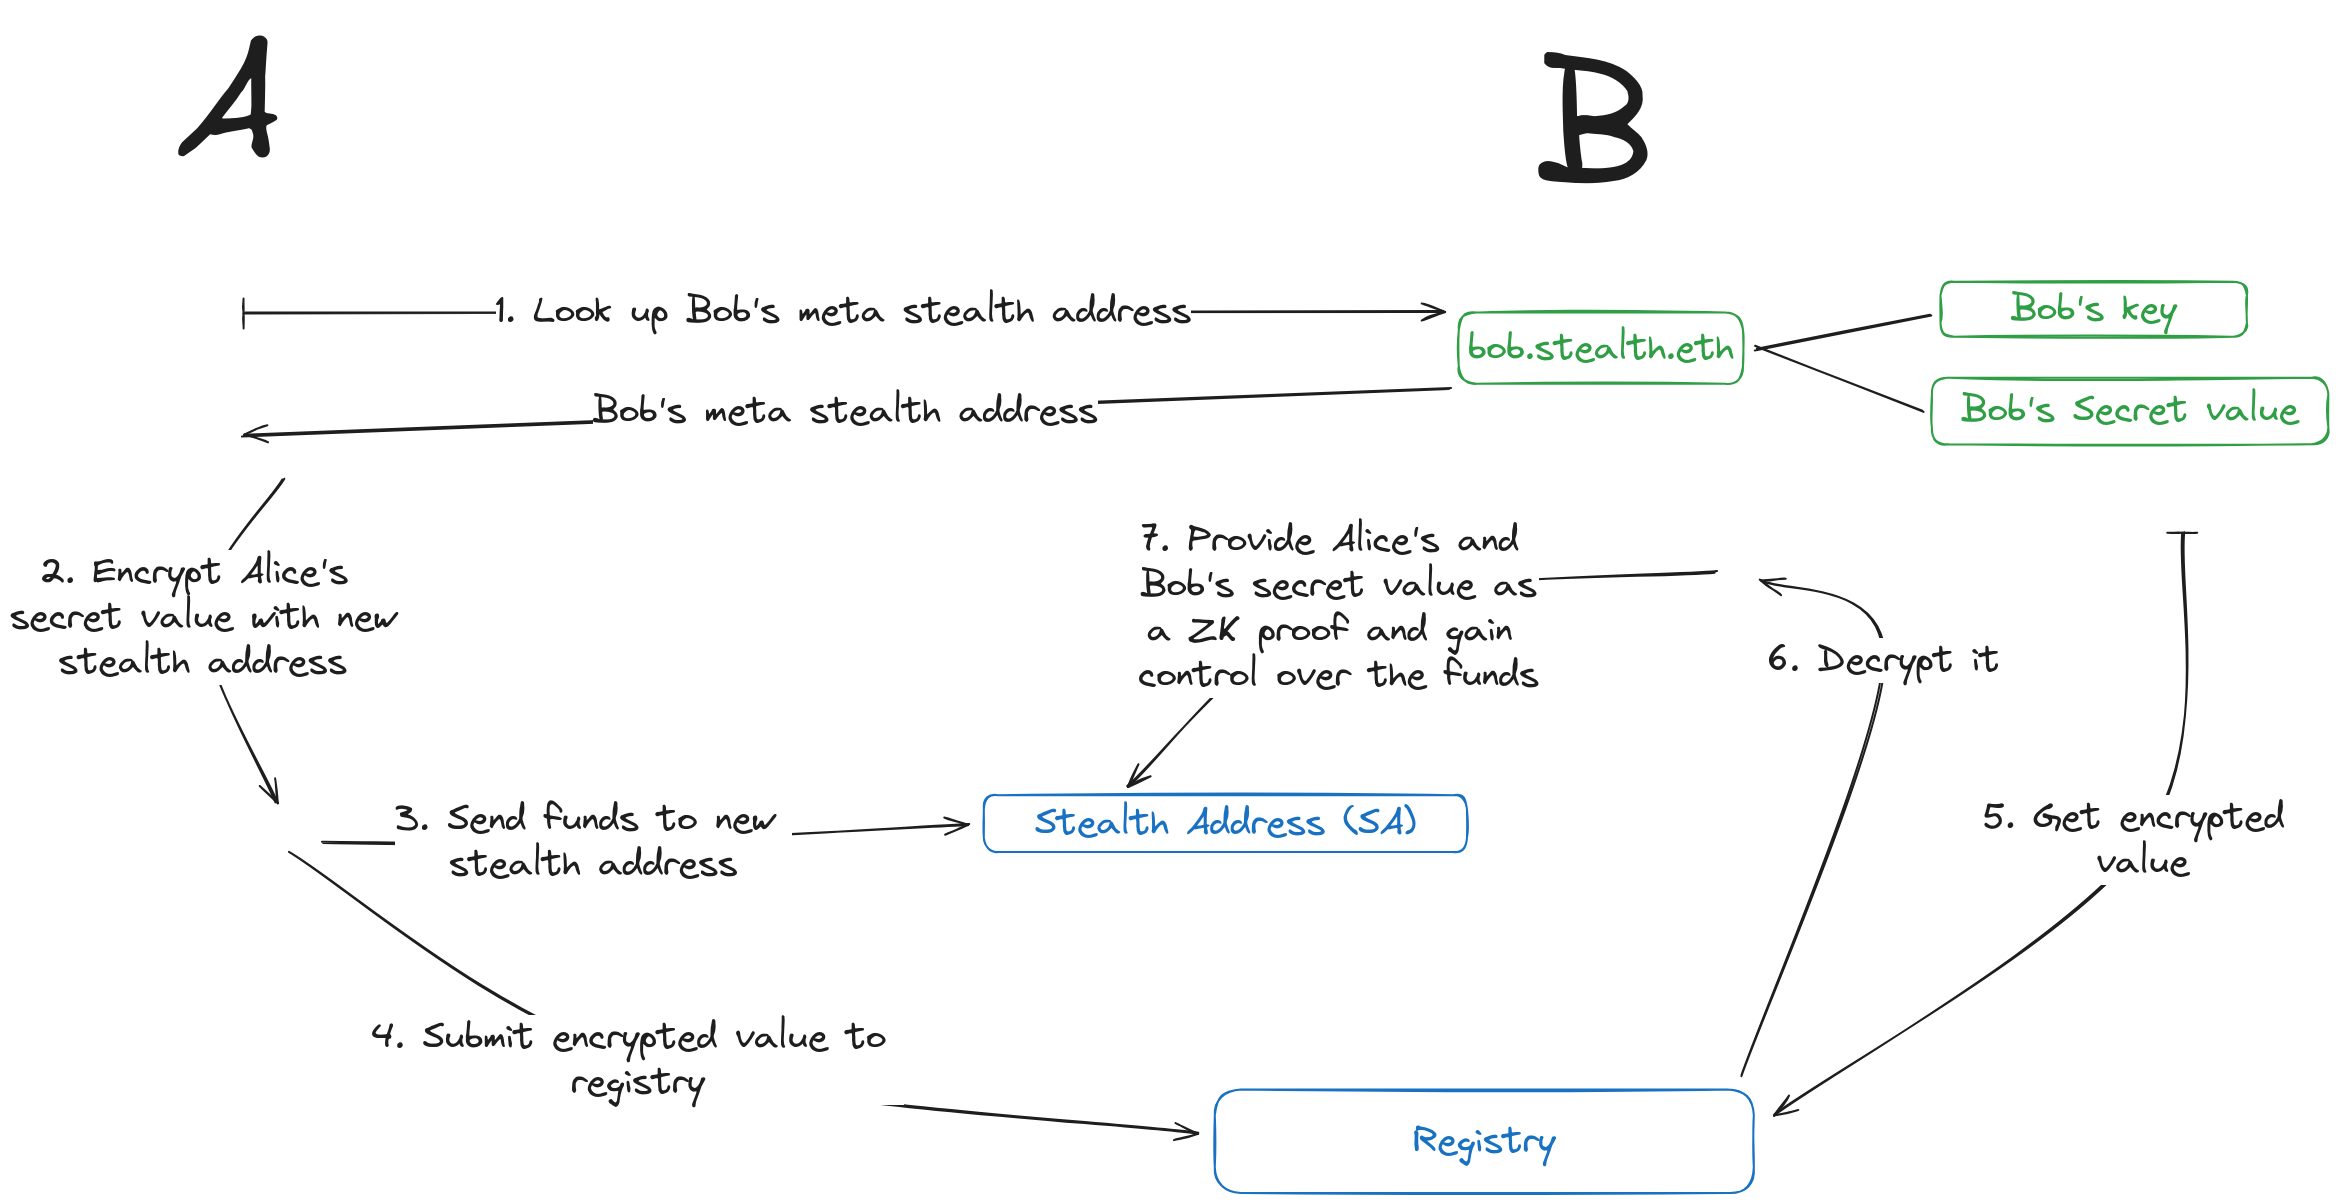
\includegraphics[scale=0.18]{assets/images/high-level.png}
    \caption{High Level Overview}
    \label{fig:hig-level}
	\cite{ButerinIncompleteGuide}
    \vspace{0.5cm}
\end{figure}

\pagebreak
\section{Initial Setup}

Before Alice can send funds to Bob, Bob must first publish his meta stealth
address to some public location. Bob computes the following:

\begin{itemize}
	\item A private key $k$,
	\item A corresponding public key $K$,
	\item A secret value $x$,
	\item A hash of the secret value $h = hash(x)$.
\end{itemize}

Bob then publishes his meta stealth address in the form of a tuple $(K, h)$.

\begin{figure}[h]
    \centering
    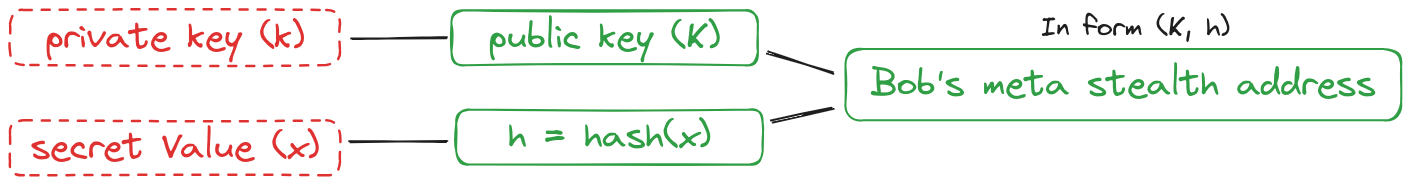
\includegraphics[scale=0.30]{assets/images/initial-setup.png}
    \caption{Initial Setup}
    \label{fig:initial-setup}
	\cite{ButerinIncompleteGuide}
    \vspace{0.5cm}
\end{figure}

\section{Sending Funds}

When Alice wishes to send funds to Bob, she queries meta stealth address registry
for Bob's meta stealth address $(K, h)$ and does the following:

\begin{itemize}
	\item Generate random secret value $c$,
    \item precompute address of the stealth address contract $sa$ \cite{stackexchangeAddressEthereum},
	\item compute $code = hash(h, c)$,
    \item deploy new stealth wallet contract with code in it,
    \item fund the deployed contract,
	\item encrypt ephemeral key $ek = encrypt(value=[c, sa], key=K)$,
    \item submit the ephemeral key to registry.
\end{itemize}

\begin{figure}[h]
    \centering
    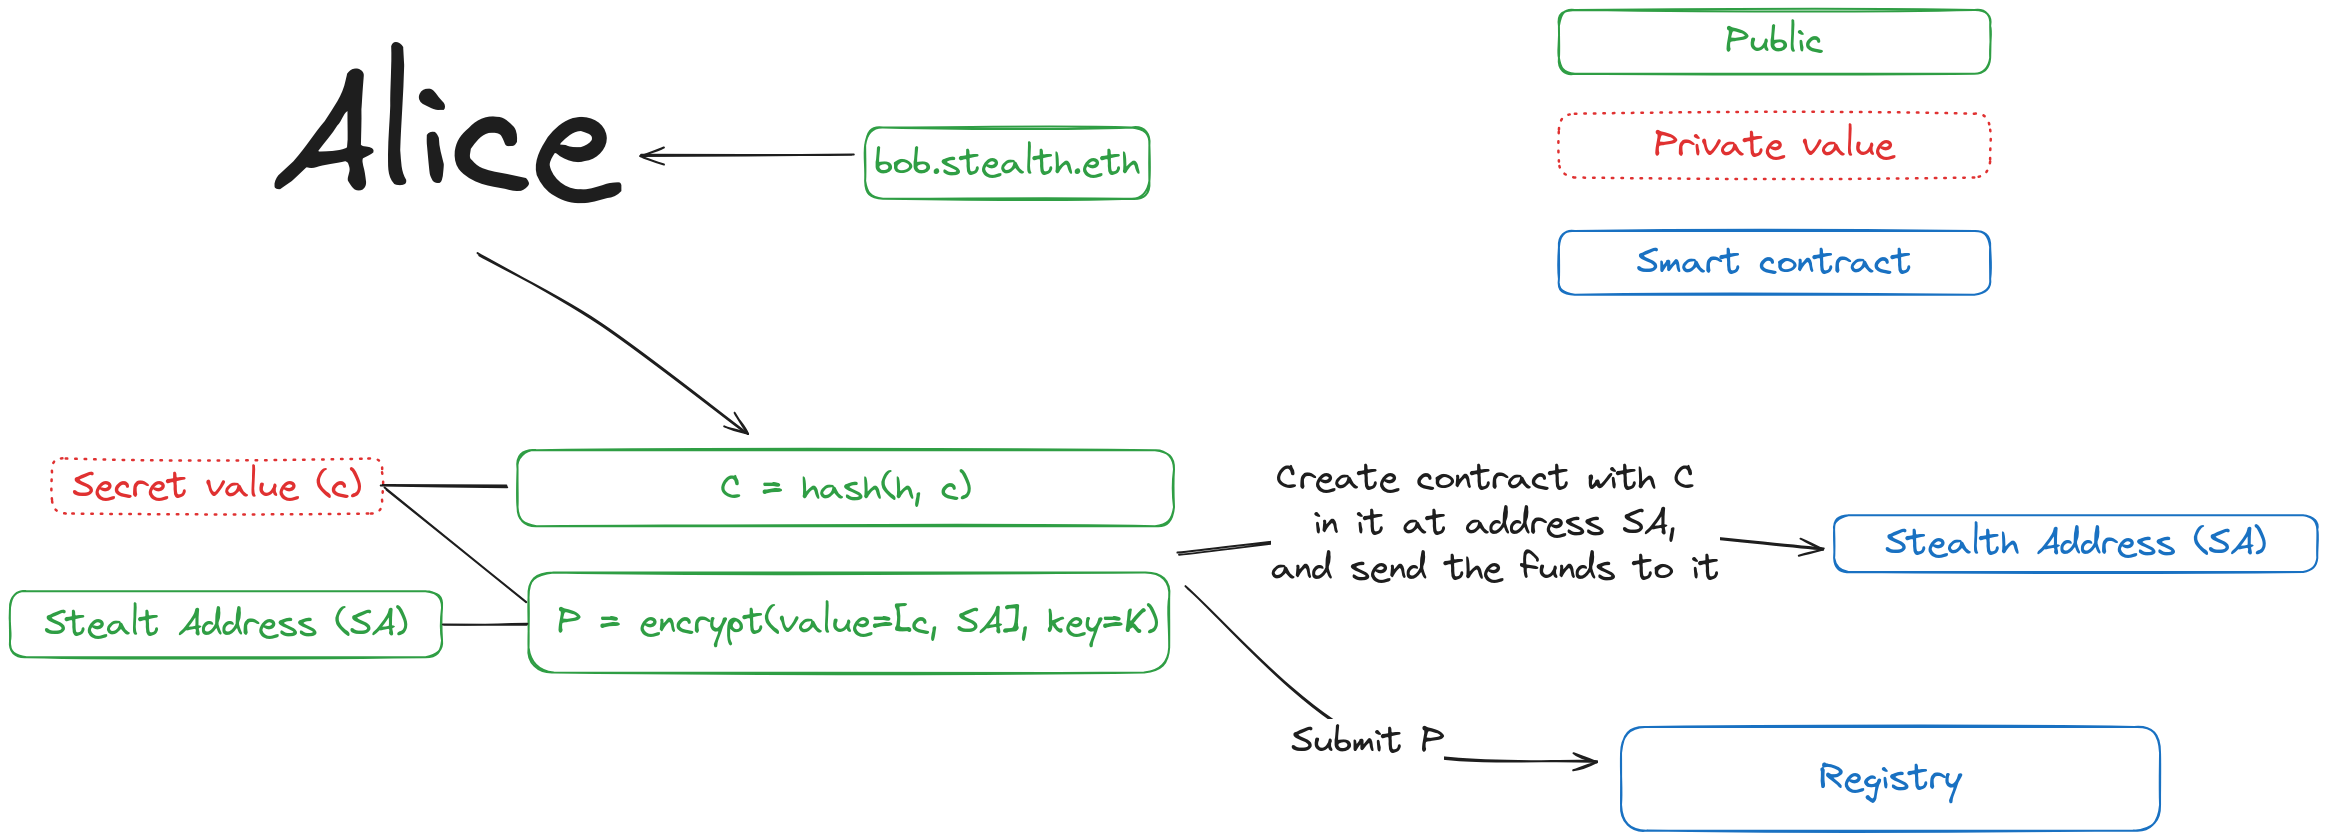
\includegraphics[scale=0.18]{assets/images/sending-funds.png}
    \caption{Sending Funds}
    \label{fig:sending-funds}
	\cite{ButerinIncompleteGuide}
    \vspace{0.5cm}
\end{figure}

\section{Scanning ephemeral keys}

Bob queries ephemeral key registry for keys from the last point he scanned.
The registry contract returns a list of ephemeral keys. Bob then tries to decrypt
each ephemeral key with his private key $k$. If the ephemeral key is meant for
Bob, then the decryption will succeed, and the decrypted value will contain
the secret value $c$ from Alice and the stealth address $sa$.

\begin{figure}[h]
    \centering
    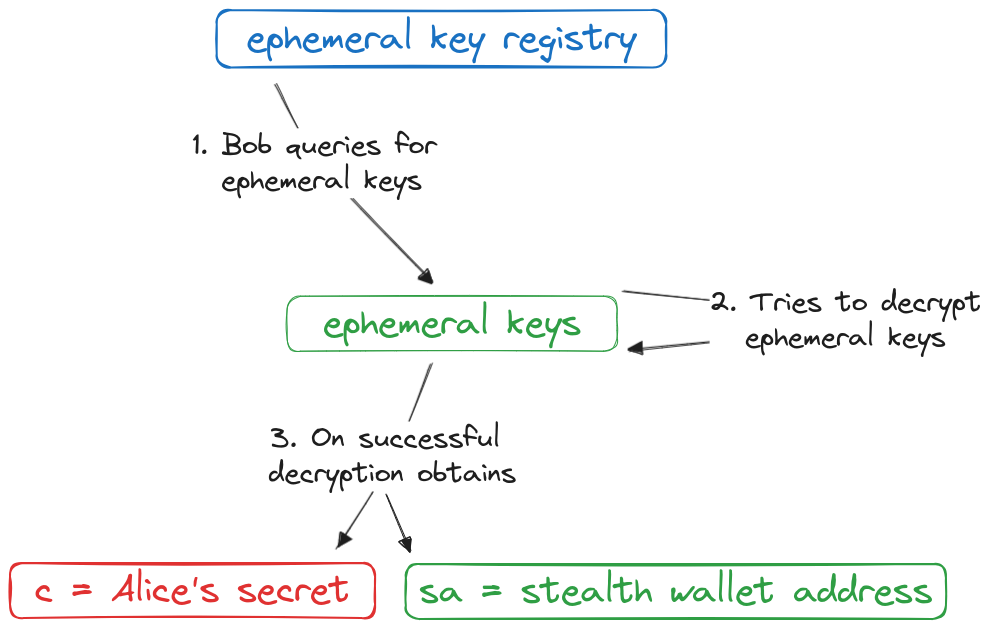
\includegraphics[scale=0.3]{assets/images/ephemeral-keys.png}
    \caption{Scanning ephemeral keys}
    \label{fig:scanning-ephemeral-keys}
    \vspace{0.5cm}
\end{figure}

\section{Gaining control of Stealth Addresses}

Bob can gain control of the stealth address $SA$ by proving to the stealth
address contract that he is the owner of the values $x$ and $c$, such that\\
$C = hash(h, c) = hash(hash(x), c)$. Bob does this by computing a ZKP for 
this statement and sending it in a transaction from any address (preferably
not from any Bob's publicly known addresses) to the stealth address $SA$. The
$SA$ contract verifies the proof and if it isn't valid, the transaction is
rejected.

\section{Overview}

The whole solution design is illustrated in Figure \ref{fig:solution},
and was inspired by the work of Vitalik Buterin\cite{ButerinIncompleteGuide}.

\begin{figure}[h]
    \centering
    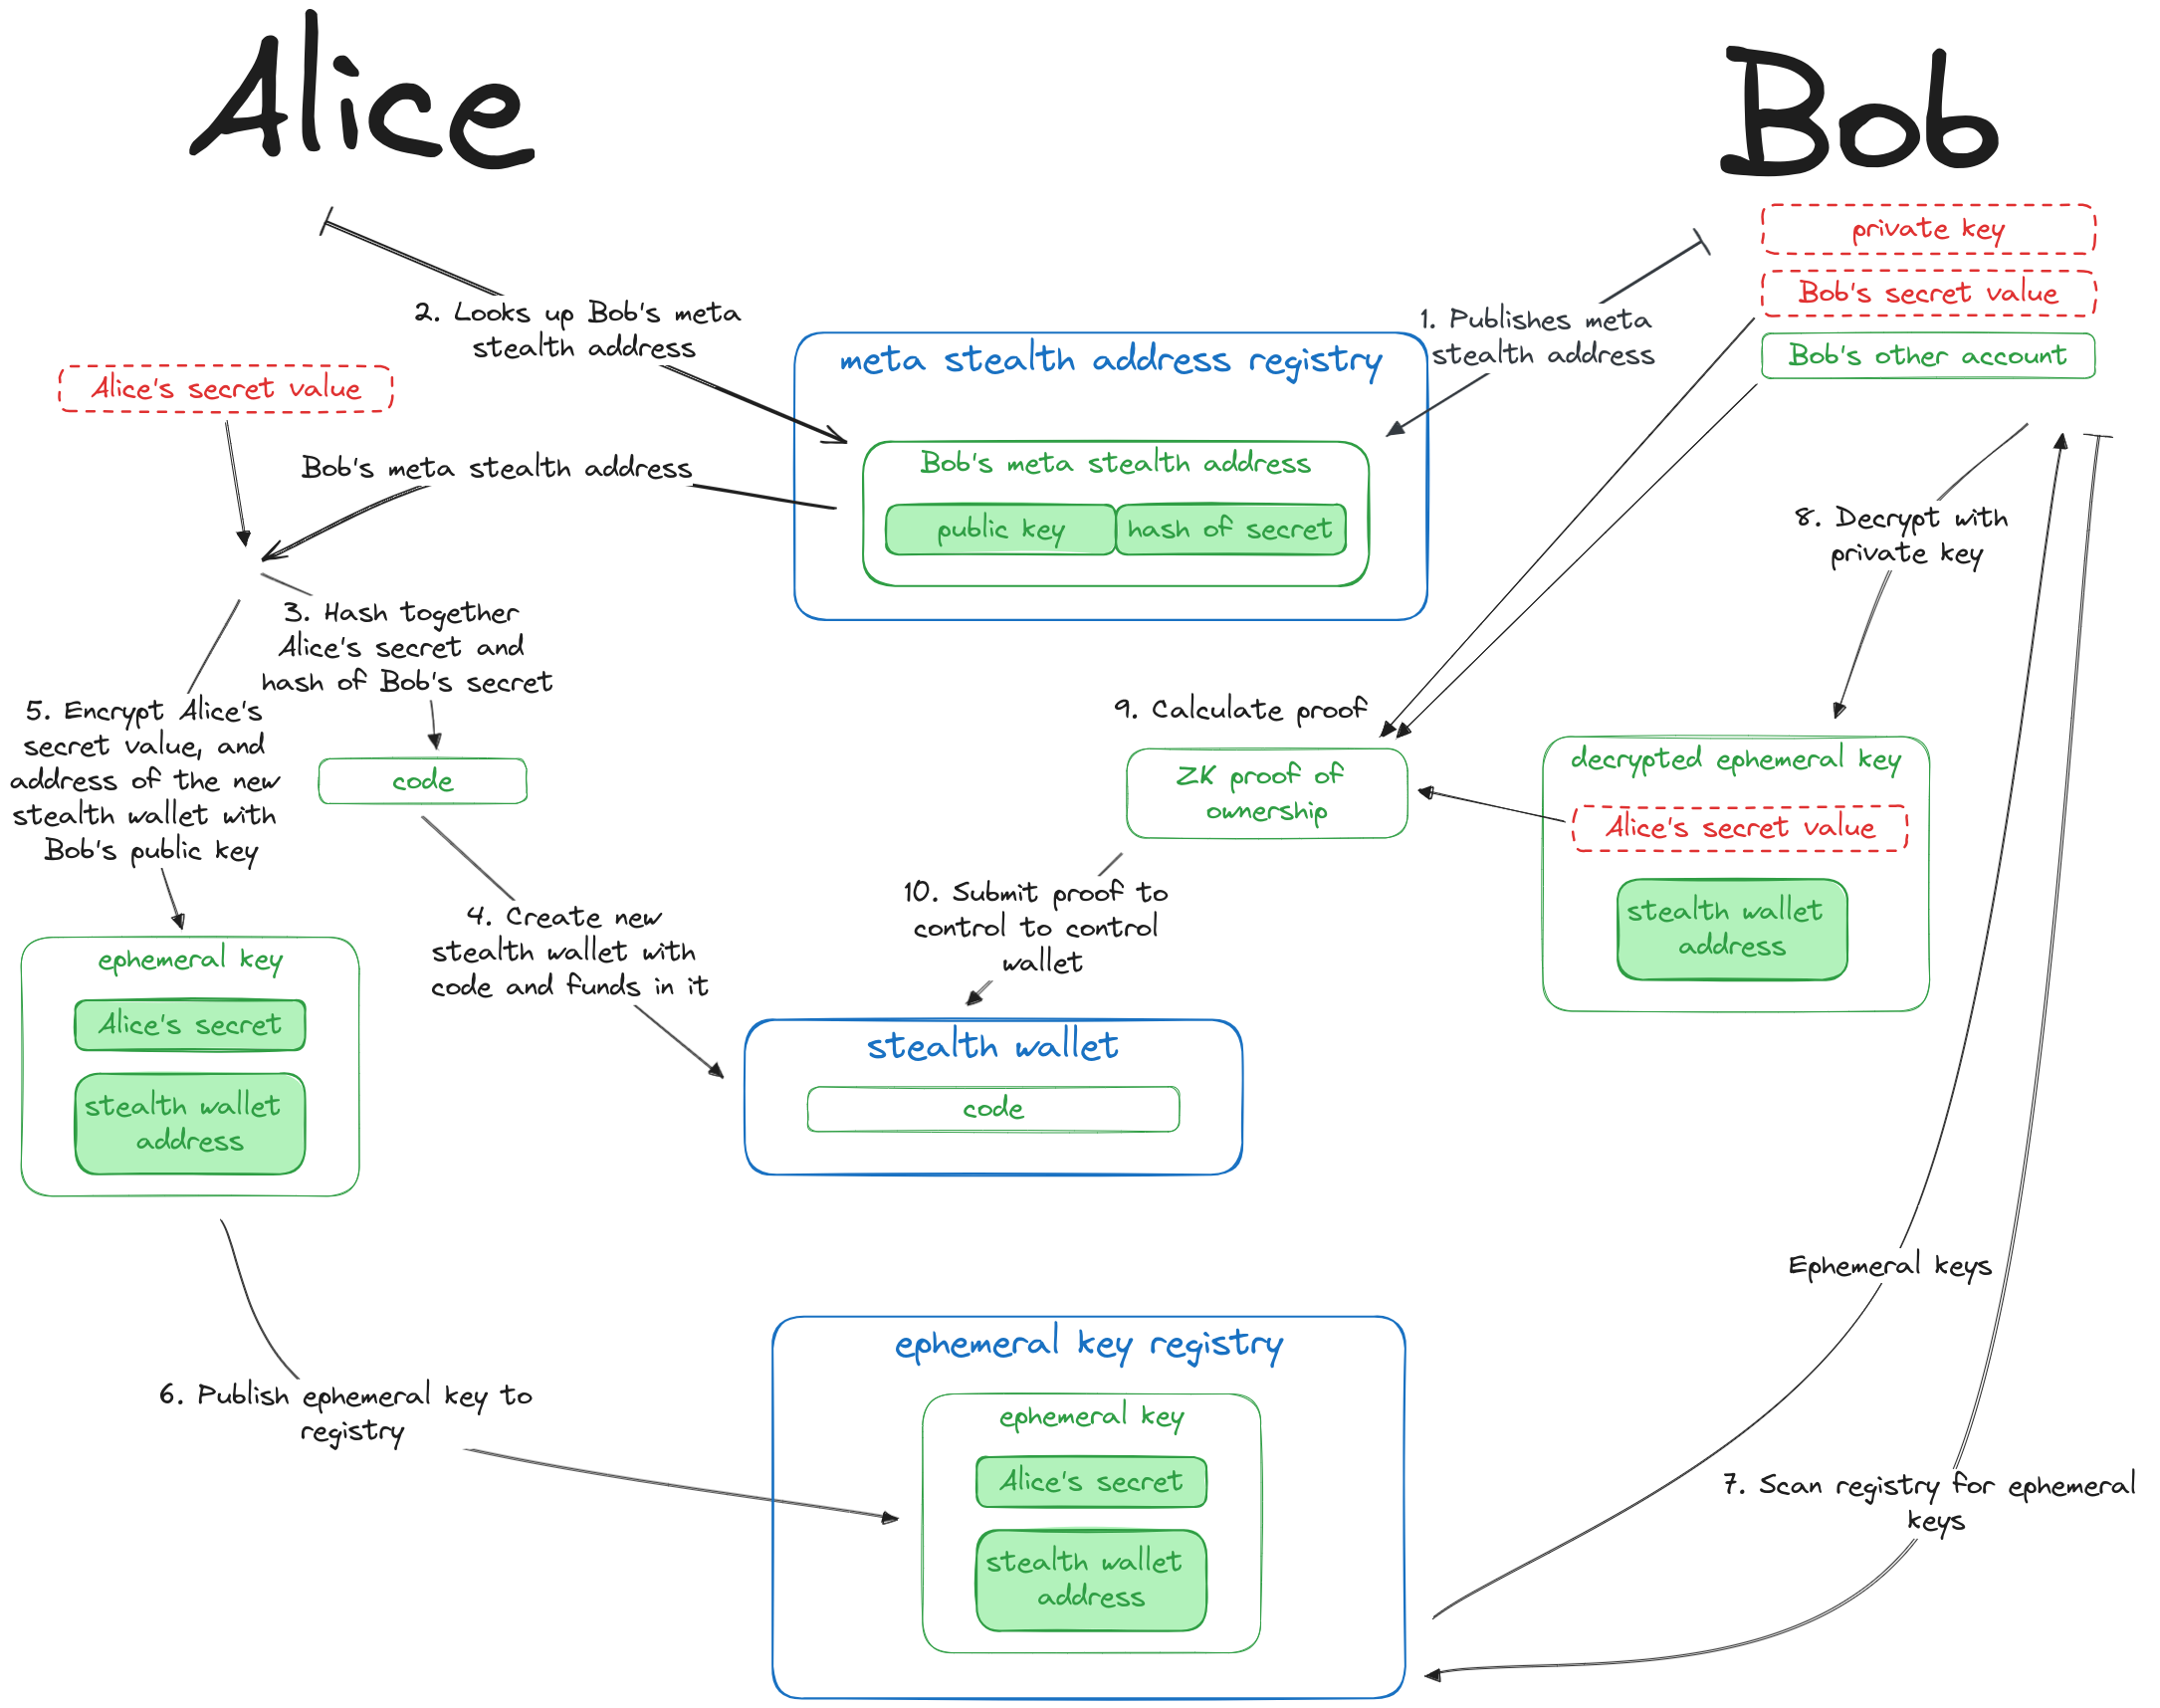
\includegraphics[width=\textwidth]{assets/images/high-level-flow.png}
    \caption{Solution Design}
	\cite{ButerinIncompleteGuide}
    \label{fig:solution}
    \vspace{0.5cm}
\end{figure}

